\documentclass{beamer}
\usepackage{mathrsfs} %Pretty fonts
\usepackage{amsmath}
\usepackage{amssymb}
\usepackage{amsfonts}

\mode<presentation>{\usetheme{Madrid}}
%%%% COMMANDS %%%%
\usepackage{xifthen}

% Real Numbers
\newcommand{\RNums}{\mathbb{R}}
% sigma-algebra
\newcommand{\salg}{\sigma\text{-algebra}}
% borel sigma-algebra
\newcommand{\borelsalg}{\mathscr{B}(\RNums)}
% Indicator function
\newcommand{\ind}{\mathbbm{1}}
% F: Sigma Algebra
\newcommand{\salgF}{\mathscr{F}}
% Probability P (P measure)
\newcommand{\Pm}{\mathbb{P}}
% Expectation's E
\newcommand{\E}{\mathbb{E}}
%Expectation with Braces
\newcommand{\Exp}[1]{\E\left[#1\right]}
% Variance
\newcommand{\V}{\mathbb{V}}
%Variance  with Braces
\newcommand{\Var}[1]{\V\left[#1\right]}
% Continuous time stochastic process
\newcommand{\ctspr}{\{X_t\}_{t\geq 0}}
% Discrete time stochastic process
\newcommand{\dtspr}{\{X_n\}_{n\geq 0}}
% Insert only one number in the "align" environment
\newcommand\numberthis{\addtocounter{equation}{1}\tag{\theequation}}
% Measure Space
\newcommand{\MeasureSpace}[1]{(\Omega, \salgF, #1)}
% Proabability Space
\newcommand{\ProbSpace}{\MeasureSpace{\Pm}}
% Norm
\newcommand{\norm}[1]{\left\lVert#1\right\rVert}
% Inner Product
\newcommand{\innerprod}[2]{\langle #1, #2\rangle}
% Family N of processes between a and b
\newcommand{\Nfam}[2]{\mathcal{N}\left[#1, #2\right]}
% Family M of processes between a and b
\newcommand{\Mfam}[2]{\mathcal{M}\left[#1, #2\right]}
%Change of Brownian motion
\newcommand{\DeltaW}[1][]{%
\ifthenelse{\isempty{#1}}{\Delta W_i}{\Delta W_#1}%
}
% differential w.r.t. the brownian motion
\newcommand{\dW}[1][]{%
\ifthenelse{\isempty{#1}}{dW}{dW_#1}%
}
% n-th partial derivative w.r.t. a single variable
\newcommand{\partialwrt}[3][]{
\ifthenelse{\isempty{#1}}
{\frac{\partial #2}{\partial #3}}
{\frac{\partial^{#1} #2}{\partial #3^{#1}}}
}

% Big-oh notation
\newcommand{\bigO}{\mathcal{O}}

% Market
\newcommand{\market}{\{X(t)\}_{t\in[0,T]}}

\title{Theoretical Grounds and Market Adaptations of Financial Fx and Interest Rate Options}
\author{Gerardo Dur\'an Mart\'in}
\institute{Universidad Marista}

\logo{
\includegraphics[height=1.7cm]{UMA_logo}}

\begin{document}
%Generates the title page
\frame{\titlepage}

\begin{frame}
	\frametitle{Table of Contents}
	\tableofcontents
\end{frame}

\section{Financial Markets}

%% Instruments
\begin{frame}
	\frametitle{Financial Markets}
	\framesubtitle{The Instruments}
	
	\begin{columns}[c]	
	
	\column{0.45\textwidth}
	\begin{itemize}
		\item <1-| alert@1> Bonds
		\item <2-| alert@2> Stocks
		\item <3-| alert@3> Foreign Exchange Currencies
		\item <4-| alert@4> Derivatives
	\end{itemize}
	
	\column{0.5\textwidth}
	\only<1>{
	A Bond is a debt obligation, its main function is to raise capital for the issuer of the bond. In turn, the buyer of the bond receives interest on the amount loaned.
	}
	\only<2>{
	A stock is a security that represents ownership on a fraction of a corporation. The return on the company for the owner of a stock is represented as a dividend.
	}
	\only<3>{
	``One country’s currency freely convertible in the foreign exchange market.'' (Kozikowski, 2013)
	}
	\only<4>{
	``[A derivative is] a financial instrument whose value depends on (or derives from) the values of other, more basic, underlying variables.'' (Hull, 2014)
	}
	\end{columns}
\end{frame}

%%Forwards
\begin{frame}
\frametitle{Financial Markets}
\framesubtitle{Derivatives: An Example}

	\begin{definition}[Forward]
		A forward is a derivative contract that gives the buyer both the right, and the obligation to to purchase a specified amount of the stock at some future time $T$ at a price $K$. The value of the forward today is 0.
	\end{definition}
	The payoff of the forward is $S_T - K$. What is the $K$ such that the contract has zero value today and has no possibility of arbitrage?
	
	\begin{figure}
	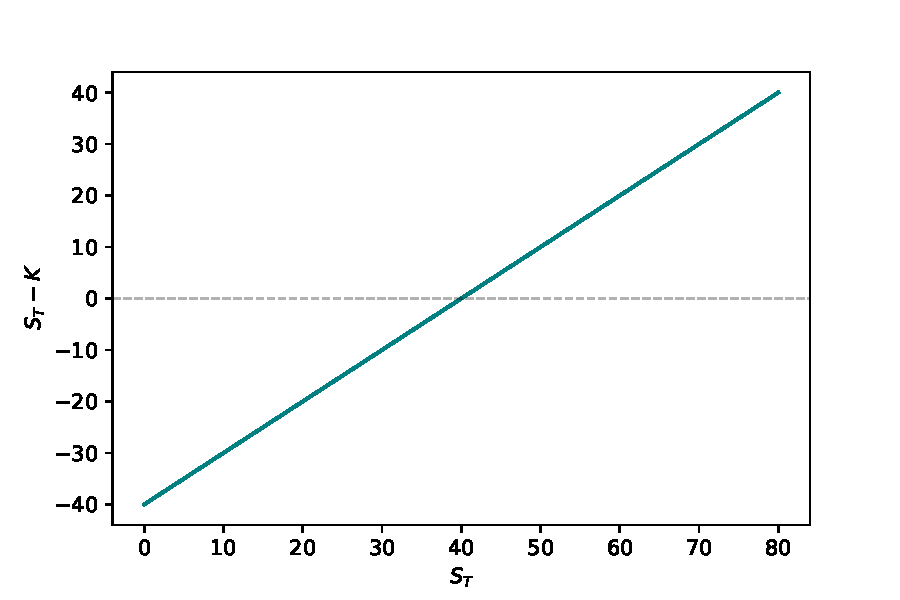
\includegraphics[width=0.45\textwidth]{../images/foward_payoff}
	\end{figure}
\end{frame}

\begin{frame}
\frametitle{Financial Markets}
\framesubtitle{Derivatives: An Example}
Assume a continuously compounded interest rate $r$, denote $S_t$ the value of the stock at time $t$. At $t=T$ the value of the forward is
$$
	S_T - K = 0
$$

By no arbitrage, the present value of the strategy is
$$
	S_0 - Ke^{-rT} = 0 \implies K = S_0e^{rT}
$$
%TODO: add why 'by no arbitrage' the latter is true.
Therefore, $S_0e^{rT}$ is the the value that guarantees no arbitrage.
\end{frame}

\section{Probability Theory}
\begin{frame}
\frametitle{Probability Theory}
We work on the measurable space
\begin{block}{Measurable Spaces}
	\[\ProbSpace\]
\end{block}

\end{frame}

\section{Brownian Motion}
\section{Stochastic Calculus}

\end{document}